\documentclass[10pt]{scrartcl}

\usepackage{scrletter}
\usepackage{parskip}

\usepackage[table]{xcolor}
\usepackage{adjustbox}
\usepackage{algorithm}
\usepackage{algpseudocode}
\usepackage{amsfonts}
\usepackage{amsmath}
\usepackage{amssymb}
\usepackage{amsthm}
\usepackage{bookmark}
\usepackage{booktabs}
\usepackage[american]{circuitikz}
\usepackage{cite}
\usepackage{fixmath}
\usepackage[acronym]{glossaries-extra}
\usepackage{hyperref}
\usepackage{import}
\usepackage{mathtools}
% \usepackage{microtype}
\usepackage[short]{optidef}
\usepackage{pgfplots}
\usepackage{ragged2e}
\usepackage[subtle]{savetrees}
\usepackage{setspace}
\usepackage{siunitx}
\usepackage{stfloats}
\usepackage[caption=false,font=footnotesize,subrefformat=parens,labelformat=parens]{subfig}
\usepackage{tabularx}
\usepackage{tikz}

\usepackage[pagewise]{lineno}
\usepackage{xr}
\externaldocument[m-]{../jsac}

% letter signature
\renewcommand*{\raggedsignature}{\raggedright}

% line referencing
\newcommand{\R}[1]{\label{#1}\linelabel{#1}} % use this to set the placement of the line reference tags
\newcommand{\lr}[1]{page~\pageref{#1}, line~\lineref{#1}} % use this to reference the tags (print line numbers)

% quoting
\newcommand\declquotedtext[2]{\expandafter\def\csname quotedtext@#1 \endcsname{#2}} % use around text you may want to quote later, but don't want printed in the main text
\newcommand\defquotedtext[2]{\declquotedtext{#1}{#2}#2} % use around text you want to appear in the main text and that you want to quote later
\newcommand\usequotedtext[1]{\csname quotedtext@#1 \endcsname} % use to print the quoted text
\newcommand{\q}[1]{“#1”} % easier way to get double quotes

\usepackage{geometry}
\usepackage[most]{tcolorbox}

% Colors
\definecolor{lightgray}{rgb}{0.9, 0.9, 0.9}
\definecolor{lightyellow}{rgb}{0.98,0.91,0.71}
\definecolor{lightred}{rgb}{0.8,0.4,0.4}

% Boxes
\newtcolorbox{replybox}{colback=lightgray, grow to right by=-2.5mm, grow to
	left by=-2.5mm, boxrule=0pt, boxsep=0pt, breakable, before skip=10pt}
\newtcolorbox{partialbox}{colback=lightyellow, grow to right by=-2.5mm, grow to
	left by=-2.5mm, boxrule=0pt, boxsep=0pt, breakable, before skip=10pt}
\newtcolorbox{todobox}{colback=lightred, grow to right by=-2.5mm, grow to left
	by=-2.5mm, boxrule=0pt, boxsep=0pt, breakable, before skip=10pt}

% Counters
\newcounter{epntcnt}
\newcounter{rpntcnt}
\newcounter{revcnt}

% Environments
\newenvironment{reviewer}{%
	\refstepcounter{revcnt}%
	\setcounter{rpntcnt}{0}%
	\section*{Reviewer \therevcnt}%
}{}
% Editor environment takes an optional argument
\newenvironment{editor}[1][Editorial Decision]{%
	\setcounter{epntcnt}{0}%
	\section*{#1}%
}{}

% Reply Commands
\newcommand{\reply}[1]{%
	\begin{replybox}%
		#1
	\end{replybox}%
}
\newcommand{\partialreply}[1]{%
	\begin{partialbox}%
		Partial reply: \emph{#1}
	\end{partialbox}%
}
\newcommand{\todoreply}[1]{%
	\begin{todobox}%
		Todo reply: \emph{#1}
	\end{todobox}%
}
\newcommand{\needsreply}{%
	\todoreply{This comment needs a reply.}%
}

% Point command differs depending on the environment
\makeatletter
\newcommand{\point}{%
	\medskip\noindent%
	\def\@tmp{editor}%
	\ifx\@tmp\@currenvir \refstepcounter{epntcnt}\theepntcnt\textbf{.}
	\else%
	\def\@tmp{reviewer}%
	\ifx\@tmp\@currenvir \refstepcounter{rpntcnt}\therpntcnt\textbf{.}
	\else\fi\fi%
}
\makeatother

% Renew the commands for the point counters to get the formatting we want in
% both the references and the item labels.
\renewcommand{\therpntcnt}{\textbf{\textup{\therevcnt.\arabic{rpntcnt}}}}
\renewcommand{\theepntcnt}{\textbf{\textup{E.\arabic{epntcnt}}}}

\setlength\parindent{0pt}
\newcommand{\bft}[1]{\mathbf{#1}}


\begin{document}

\setkomavar{date}{\today}
\setkomavar{signature}{Yang Zhao}
\setkomavar{subject}{Re: Minor amendments on thesis ``Reconfigurable Intelligent Surfaces: Beamforming, Modulation, and Channel Shaping''}

\begin{letter}{%
		Prof Geoffrey Ye Li\\
		Department of Electrical and Electronic Engineering\\
		Imperial College London
	}
	\opening{Dear Prof Li,}
	% Thank you for your time and effort in reviewing my thesis
	I would like to express my sincere gratitude to you and Dr Yuan Ding for reviewing my thesis and providing valuable comments, which helped me to improve the quality of the manuscript significantly.
	% I would like to express my sincere gratitude to you for the valuable comments and suggestions, which helped us improve the quality of the manuscript significantly.
	Below is a point-to-point response highlighting all the changes made to the manuscript.
	I hope that the revisions and clarifications make the thesis meet the PhD standards at Imperial.
	\closing{Yours sincerely,}
\end{letter}

\begin{reviewer}
	\point A few typos and run-on sentences. They were marked in the printed thesis which was left with the student.
	\reply {
		Thank you for reading carefully and pointing out the issues. I have carefully proofread the thesis again and corrected all the grammar issues.
		Besides, I noticed many handwritten questions and comments in the printed thesis, which are not included in the official review report.
		Those have also been addressed in the revised manuscript (mostly in terms of footnotes).
	}

	\point Why RIS elements need to be non-resonant and sub-wavelength?
	\reply {
		We have added a bullet point in Chapter 1 to explain the importance of non-resonant and sub-wavelength RIS elements. That is,
		\begin{itemize}
			\item \emph{Non-resonant and sub-wavelength:} Instead of relying on the resonance effect at a specific frequency, RIS ideally functions as a universal scatterer serving a wide range of frequency bands with independent response control. Miniature elements with sub-wavelength dimension and spacing further reduces mutual coupling and improves spatial resolution. However, they pose a great challenge on the design and optimization of the circuit components and matching network.
		\end{itemize}
	}

	\point  Why only reflection is considered, but not transmission? This needs to be clarified.
	\reply {
		It is worth noticing that refraction and reflection are different forms of {wave scattering} where the signal amplitude and phase are altered by the metamaterial.
		Their contributions can be jointly modeled within the scattering matrix $\mathbf{\Theta}$, which corresponds to the $S$-parameters in microwave engineering and the channel matrix in wireless communications.
	}

	\point As for the non-symmetric BD-RIS, it is better to present and discuss an example to
	justify this.
	\reply {
		We have added the following arguments in Chapter 2 to discuss the implementation of asymmetric BD-RIS.

		On the other hand, lossless networks may also be built over asymmetric passive components (e.g., ring hybrids and branch-line hybrids) such that the symmetric constraint (2.8a) can be relaxed.
		A 4-port ring hybrid is illustrated in Fig. \ref{fg:ring_hybrid}.
		\begin{figure}[H]
			\centering
			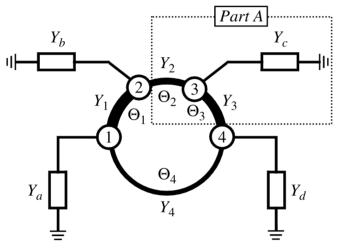
\includegraphics[width=0.5\textwidth]{../assets/chapter_2/ring_hybrid.pdf}
			\caption{A 4-port asymmetric ring hybrid. Here the arc length between ports are $\Theta_1 = \Theta_2 = \Theta_3 = \lambda / 4$ and $\Theta_4 = 3 \lambda / 4$ where $\lambda$ is the wavelength. The termination admittances $Y_a$ to $Y_d$ are arbitrary and the characteristic admittances of transmission-line sections are not necessarily the same, such that the scattering parameters can be asymmetric. Source: modified from [3].}
			\label{fg:ring_hybrid}
		\end{figure}

		By reconfiguring passive asymmetric components, we end up with the ultimate passive model where energy conservation (2.8b) is the only constraint for each group, as has been widely adopted in quantum physics.
	}

	\point Need to clarify why deterministic multi-sine is better than modulated multi-carrier signals for wireless power transfer?
	\reply {
		We have added the reasoning in Chapter 3 as below.

		Following [73], we superpose a multi-carrier modulated information-bearing waveform to an unmodulated power-dedicated multisine to boost the spectrum and energy efficiency.
		It is worth mentioning that the latter is beneficial for WPT due to its higher PAPR (as discussed in Section 2.2.3.2) and better high-order statistics on expectation (c.f. (3.9b) and (3.9d) in Section 3.2.6).
	}

	\point Will superimposed multi-sine saturate receiver, so that the baseband model cannot
	be used?
	\reply {
		This is a very good point. We have added the following paragraph in Chapter 3 to discuss the receiver saturation issue.

		A major benefit of the superposed waveform is that the multisine is deterministic and its impact on WIT can be completely eliminated by waveform cancellation or translated demodulation [73].
		The former is achieved by subtracting the multisine from the received signal at additional signal processing cost, while the latter requires a demodulator with higher saturation power level.
	}

	\point As for one of the simulation that 40dBm EIRP is used, could we use lower (within regulation limit) power for same conclusion?
	\reply {
		This is indeed a practical issue since the regulation for EIRP is 36 dBm in the 2.4 GHz band.
		I am totally sure that reducing the EIRP by 4dB will only affect the scale of the simulation results without altering any conclusion in Chapter 3.
		Unfortunately, my access to HPC resources at Imperial has been revoked after the registration period, and re-running all codes on my laptop is too time-consuming.
		I have added a footnote in Chapter 3 on this point and published the corrected source code online for everyone to verify the results.
		% In the revised manuscript, EIRP has been reduced to 36 dBm and relevant simulation results have been updated accordingly. We notice that all conclusions in Chapter 3 remain valid.
	}

	\point The pathloss exponent changes at 12 meters, which makes the simulation model not generic to reveal the benefit of employing RIS.
	\reply {
		This is indeed a special modeling choice that simulates an indoor environment where two rooms are connected by a RIS door. The benefits of employing RIS remain valid under different path loss models, as investigated in Chapters 4 and 5.
		We have added the following explanation in Chapter 3.

		We consider a Wi-Fi-like environment at center frequency \qty{2.4}{\GHz} where the channel follows IEEE TGn channel model D [131]. To simulate an indoor environment where two rooms are separated by a wall and a RIS door, we set the path loss exponent to \num{2} up to \qty{10}{\meter} and \num{3.5} onwards to penalize the penetration loss.
	}

	\point For SWIPT, why we only discuss TS and PS, but not FS?
	\reply {
		Frequency Selection (FS) is a practical SWIPT strategy whose R-E performance is strictly dominated by PS.
		We have added the following footnote in Chapter 3 to discuss this.

		It is worth mentioning that many other SWIPT transceiving strategies have been proposed in the literature. In particular, frequency selection is more practical where multisine is used over $n$ subbands and information is carried over the remaining $N-n$ subbands, where $n$ is a design parameter. This can be viewed as a special case of PS and its R-E region is strictly contained with that of the latter, such that we don't include a special study in this work.
	}

	\point $x_k$: need to justify the assumption of coherent channel block is large then BB.
	\reply {
		In the revised Chapter 4, we have emphasized the assumption when discussing Fig. 4.2(a) and introducing the signal model. The following sentence has been added.


		We assume the coherent channel block is longer than backscatter symbol block, and the backscatter symbol block is longer than primary symbol block.


		We assume the channel coherence time is longer than the backscatter symbol duration, \textellipsis
	}
\end{reviewer}

\end{document}
